% Created 2024-04-21 Sun 21:49
% Intended LaTeX compiler: pdflatex
\documentclass[presentation]{beamer}
\usepackage[utf8]{inputenc}
\usepackage[T1]{fontenc}
\usepackage{graphicx}
\usepackage{longtable}
\usepackage{wrapfig}
\usepackage{rotating}
\usepackage[normalem]{ulem}
\usepackage{amsmath}
\usepackage{amssymb}
\usepackage{capt-of}
\usepackage{hyperref}
\mode<beamer>{\usetheme{Madrid}}
\definecolor{SUred}{rgb}{0.59375, 0, 0.17969} % SU red (primary)
\definecolor{SUblue}{rgb}{0, 0.17578, 0.38281} % SU blue (secondary)
\setbeamercolor{palette primary}{bg=SUred,fg=white}
\setbeamercolor{palette secondary}{bg=SUblue,fg=white}
\setbeamercolor{palette tertiary}{bg=SUblue,fg=white}
\setbeamercolor{palette quaternary}{bg=SUblue,fg=white}
\setbeamercolor{structure}{fg=SUblue} % itemize, enumerate, etc
\setbeamercolor{section in toc}{fg=SUblue} % TOC sections
% Override palette coloring with secondary
\setbeamercolor{subsection in head/foot}{bg=SUblue,fg=white}
\setbeamercolor{date in head/foot}{bg=SUblue,fg=white}
\institute[SU]{Shenandoah University}
\titlegraphic{\includegraphics[width=0.5\textwidth]{\string~/Documents/suLogo/suLogo.pdf}}
\newcommand{\R}{\mathbb{R}}
\usepackage{tikz}
\usepackage{pgfplots}
\usetheme{default}
\author{Chase Mathison\thanks{cmathiso@su.edu}}
\date{22 April 2024}
\title{More Ellipses}
\hypersetup{
 pdfauthor={Chase Mathison},
 pdftitle={More Ellipses},
 pdfkeywords={},
 pdfsubject={},
 pdfcreator={Emacs 29.1 (Org mode 9.6.7)}, 
 pdflang={English}}
\begin{document}

\maketitle

\section{Announcements}
\label{sec:orgda77369}
\begin{frame}[label={sec:orgfebf85e}]{Announcements}
\begin{enumerate}
\item Homework due tonight.
\item Project.
\item No office hours today.
\end{enumerate}
\end{frame}


\section{Lecture}
\label{sec:orgaecb6e8}
\begin{frame}[label={sec:org33886ff}]{General Ellipse}
Let's look at the equation of a general ellipse centered at the point \(\left( h,k \right)\).

\vspace{10in}
\end{frame}

\begin{frame}[label={sec:org57ae33b}]{Facts about General Ellipses}
\begin{center}
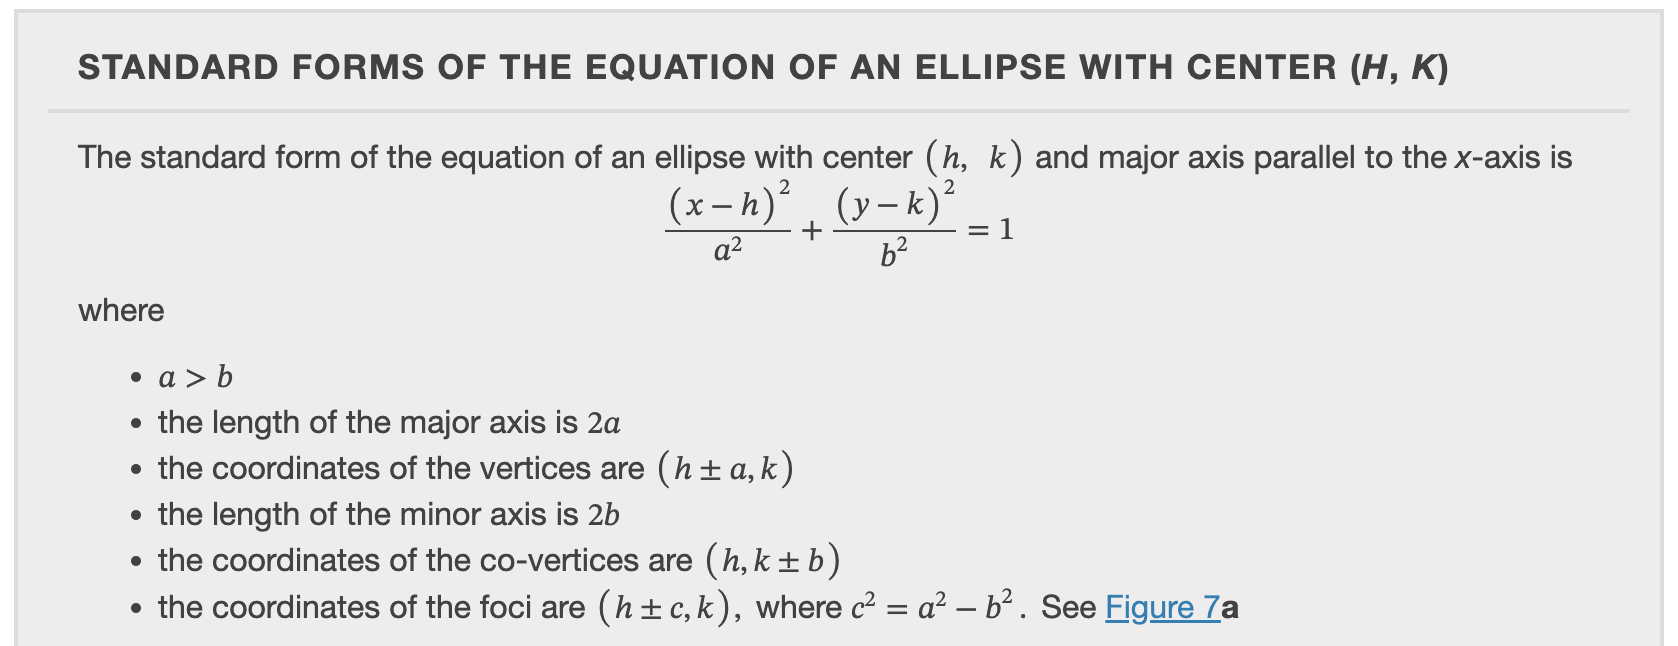
\includegraphics[width=0.8\textwidth]{./gel001.png}
\end{center}
\end{frame}

\begin{frame}[label={sec:org5c1042e}]{Facts about General Ellipses}
\begin{center}
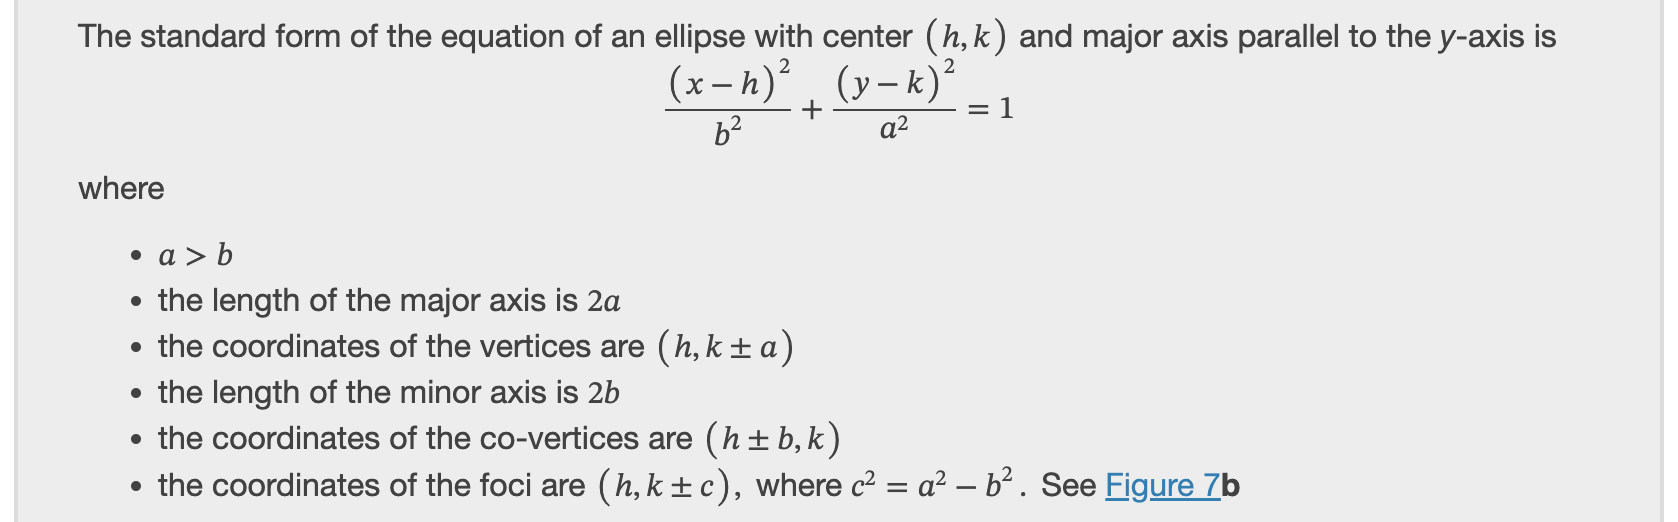
\includegraphics[width=0.8\textwidth]{./gel002.png}
\end{center}
\end{frame}

\begin{frame}[label={sec:orgadca5ed}]{Facts about General Ellipses}
\begin{center}
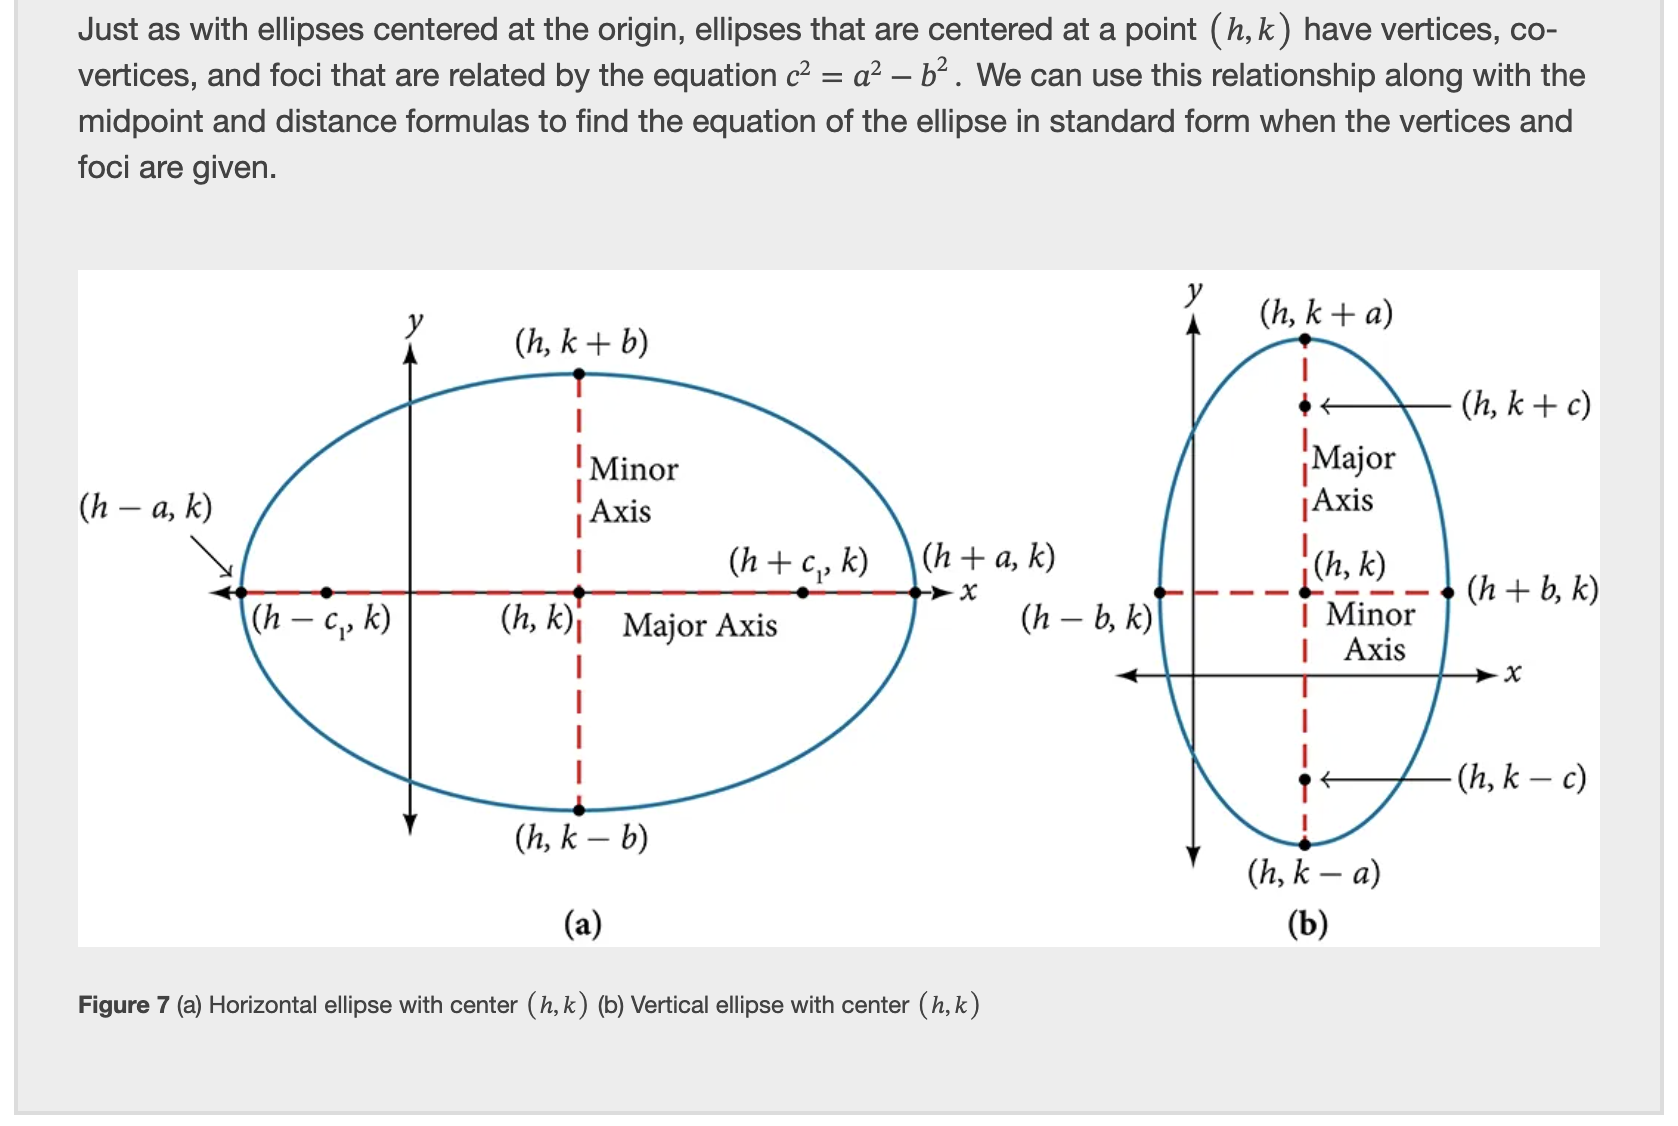
\includegraphics[width=0.8\textwidth]{./gel003.png}
\end{center}
\end{frame}

\begin{frame}[label={sec:org0474946}]{Example}
Let's plot the ellipse given by the equation

\[
\frac{\left( x-1 \right)^2}{16} + \frac{\left( y+2 \right)^2}{4} = 1\]

\begin{tikzpicture}
  \begin{axis}[axis lines = center,
    xmin=-8,
    xmax=8,
    ymin=-8,
    ymax=8,
    xtick distance = 1,
    ytick distance = 2,
    xlabel={$x$},
    ylabel={$y$}]
    
  \end{axis}
\end{tikzpicture}
\end{frame}

\begin{frame}[label={sec:org654bc6e}]{Example}
What is the equation of the ellipse with this graph:

\begin{tikzpicture}
  \begin{axis}[axis lines = center,
    xmin=-8,
    xmax=8,
    ymin=-8,
    ymax=8,
    xtick distance = 1,
    ytick distance = 2,
    xlabel={$x$},
    ylabel={$y$}]
    \addplot[domain=3:7,samples=100,color=blue]{2+3*sqrt(1-(x-5)^2/4)};
    \addplot[domain=3:7,samples=100,color=blue]{2-3*sqrt(1-(x-5)^2/4)};    
  \end{axis}
\end{tikzpicture}
\end{frame}

\begin{frame}[label={sec:org69b25a8}]{Example}
\end{frame}

\begin{frame}[label={sec:org44a3b6d}]{Completing the square}
Is the following equation the equation of an ellipse?

\[
9x^2+36x+4y^2-32y + 100 = 36\]

What about

\[
9x^2+36x-4y^2-32y + 100 = 36\]

Let's look at how we can see!
\end{frame}

\begin{frame}[label={sec:orgbaa6279}]{Completing the square}
Let's begin with the first example.
\[
9x^2+36x+4y^2-32y + 100 = 36\]

\vspace{10in}
\end{frame}

\begin{frame}[label={sec:orgc9071a1}]{Example}
\end{frame}

\begin{frame}[label={sec:org14032d2}]{Example}
\end{frame}

\begin{frame}[label={sec:orgc29bf7c}]{Example}
Now let's check if

\[
9x^2+36x-4y^2-32y + 100 = 36\]

is the equation of an ellipse.

\vspace{10in}
\end{frame}
\end{document}